\section{Período}
\label{sec:Periodo}
\index{Música!Período}



Um período é geralmente formado por duas frases \cite[pp. 350]{duckworth2007creative} \cite[pp. 336]{medteoria};
quando este é o caso 
\begin{itemize}  
\item a primeira é chamada frase antecedente e 
\item a segunda de frase consequente.
\end{itemize}

A frase consequente é uma repetição modificada da frase antecedente 
\cite[pp. 53,55]{schoenberg1990fundamentos} \cite[pp. 25,29]{schoenberg1967fundamentals},
de modo que esta geralmente inicia com o mesmo motivo básico que a frase anterior,
com uma possível leve modificação na melodia
\cite[pp. 51]{schoenberg1990fundamentos} \cite[pp. 25]{schoenberg1967fundamentals};
por outro lado, também é possível que só a estrutura rítmica seja preservada,
e importantes mudanças nas alturas das notas sejam feitas
\cite[pp. 57]{schoenberg1990fundamentos} \cite[pp. 30]{schoenberg1967fundamentals}.


A frase antecedente termina deixando uma sensação de um final aberto, 
que é solucionado pela segunda frase que finaliza com uma cadência conclusiva;
ou seja o período tem duas cadencias uma fraca para a frase antecedente e 
outra forte para a frase consequente 
\cite[pp. 350]{duckworth2007creative} \cite[pp. 336]{medteoria} \cite[pp. 1176]{latham2008diccionario}
\cite[pp. 25,29]{schoenberg1967fundamentals}.

Estas duas frases geram uma analogia literária de pergunta e resposta, respectivamente \cite[pp. 336]{medteoria}.
Comumente, um período é composto por 8 compassos com frases de 4 compassos cada uma \cite[pp. 25]{schoenberg1967fundamentals}.

A Figura \ref{fig:periodostruct} mostra a estrutura de uma período. 
\begin{figure}[!h]
  \centering
    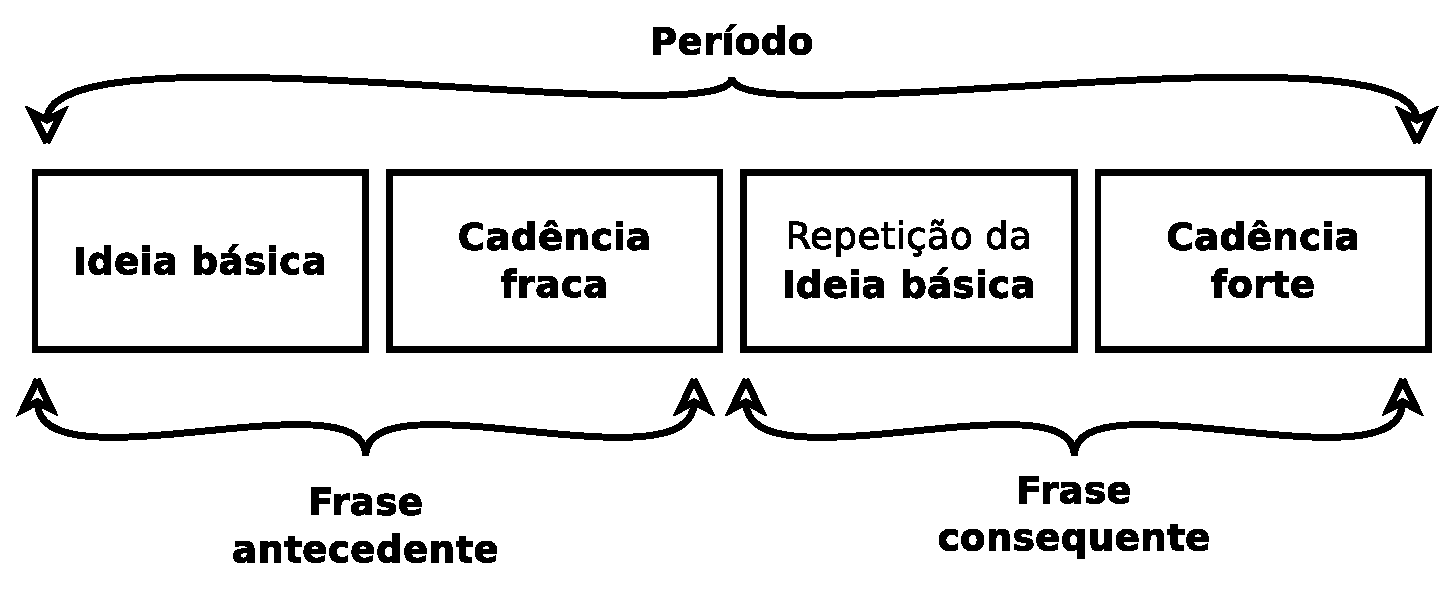
\includegraphics[width=\textwidth]{chapters/cap-musica-composer/periodo.eps}
\caption{Estrutura de uma sentença.}
\label{fig:periodostruct}
\end{figure}

\begin{example}
Na sinfonia no. 9 de Ludwig van Beethoven podemos achar exemplos do uso de períodos. 
Na Figura \ref{fig:periodo-ex1} podemos ver um período formado por 8 compassos desta sinfonia;
os 4 primeiros compassos correspondem à frase antecedente 
e os 4 últimos à frase consequente.
\end{example}

\begin{figure}[!h]
  \centering
    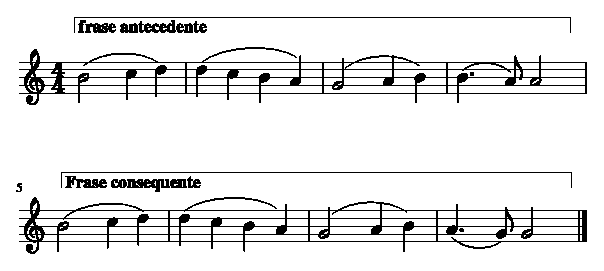
\includegraphics[width=\textwidth]{chapters/cap-musica-composer/periodo-ex1-1.eps}
\caption{Oito compassos da sinfonia no. 9, de Ludwig van Beethoven.}
\label{fig:periodo-ex1}
\end{figure}


